A análise experimental foi realizada gerando os sinais que correspondem à seguinte função:

\begin{align}
    x(t) = \cos{2\pi 100 t} + 3 \cos{2\pi 250 t} + \\
    5 \cos{2\pi 750 t} + 7 \cos(2\pi 1000 t)    
\end{align}

Assim sendo, para gerar o sinal, foi desenvolvida uma função chamada \textit{generateSignal}, que irá gerar um sinal com frequência de amostragem igual a $2500\, \text{Hz}$.

\markdownInput{03_experimental_analysis/signal_gen.md}

\subsubsection*{Valores esperados no Eixo da Frequência (em Hz)}

Considerando que a função $x(t)$ é composta por cossenos com frequências $100 \, \text{Hz}$, $250 \, \text{Hz}$, $750 \, \text{Hz}$ e $1000 \, \text{Hz}$, espera-se que as magnitudes dos coeficientes da DFT apresentem picos nestas frequências.

Portanto, espera-se que em cada frequência do espectro sejam observados picos de amplitude proporcionais aos coeficientes de cada componente da função $x(t)$. Os valores esperados são:

\begin{itemize}
    \item \textbf{Frequência: $100 \, \text{Hz}$} — Pico na amplitude do coeficiente correspondente.
    \item \textbf{Frequência: $250 \, \text{Hz}$} — Pico na amplitude 3 vezes maior que o do cosseno de $100 \, \text{Hz}$.
    \item \textbf{Frequência: $750 \, \text{Hz}$} — Pico na amplitude 5 vezes maior que o do cosseno de $100 \, \text{Hz}$.
    \item \textbf{Frequência: $1000 \, \text{Hz}$} — Pico na amplitude 7 vezes maior que o do cosseno de $100 \, \text{Hz}$.
\end{itemize}

\subsection{Questões}
Amostre o sinal  a um período de amostragem e determine os seguintes:

\subsubsection*{(a) \textbf{(1,0 pontos) }}
Calcule a DFT e FFT do sinal amostrado com uma janela de somente 32 amostras. É possível observar no espectro as senóides?

\begin{figure}[H]
    \centering
    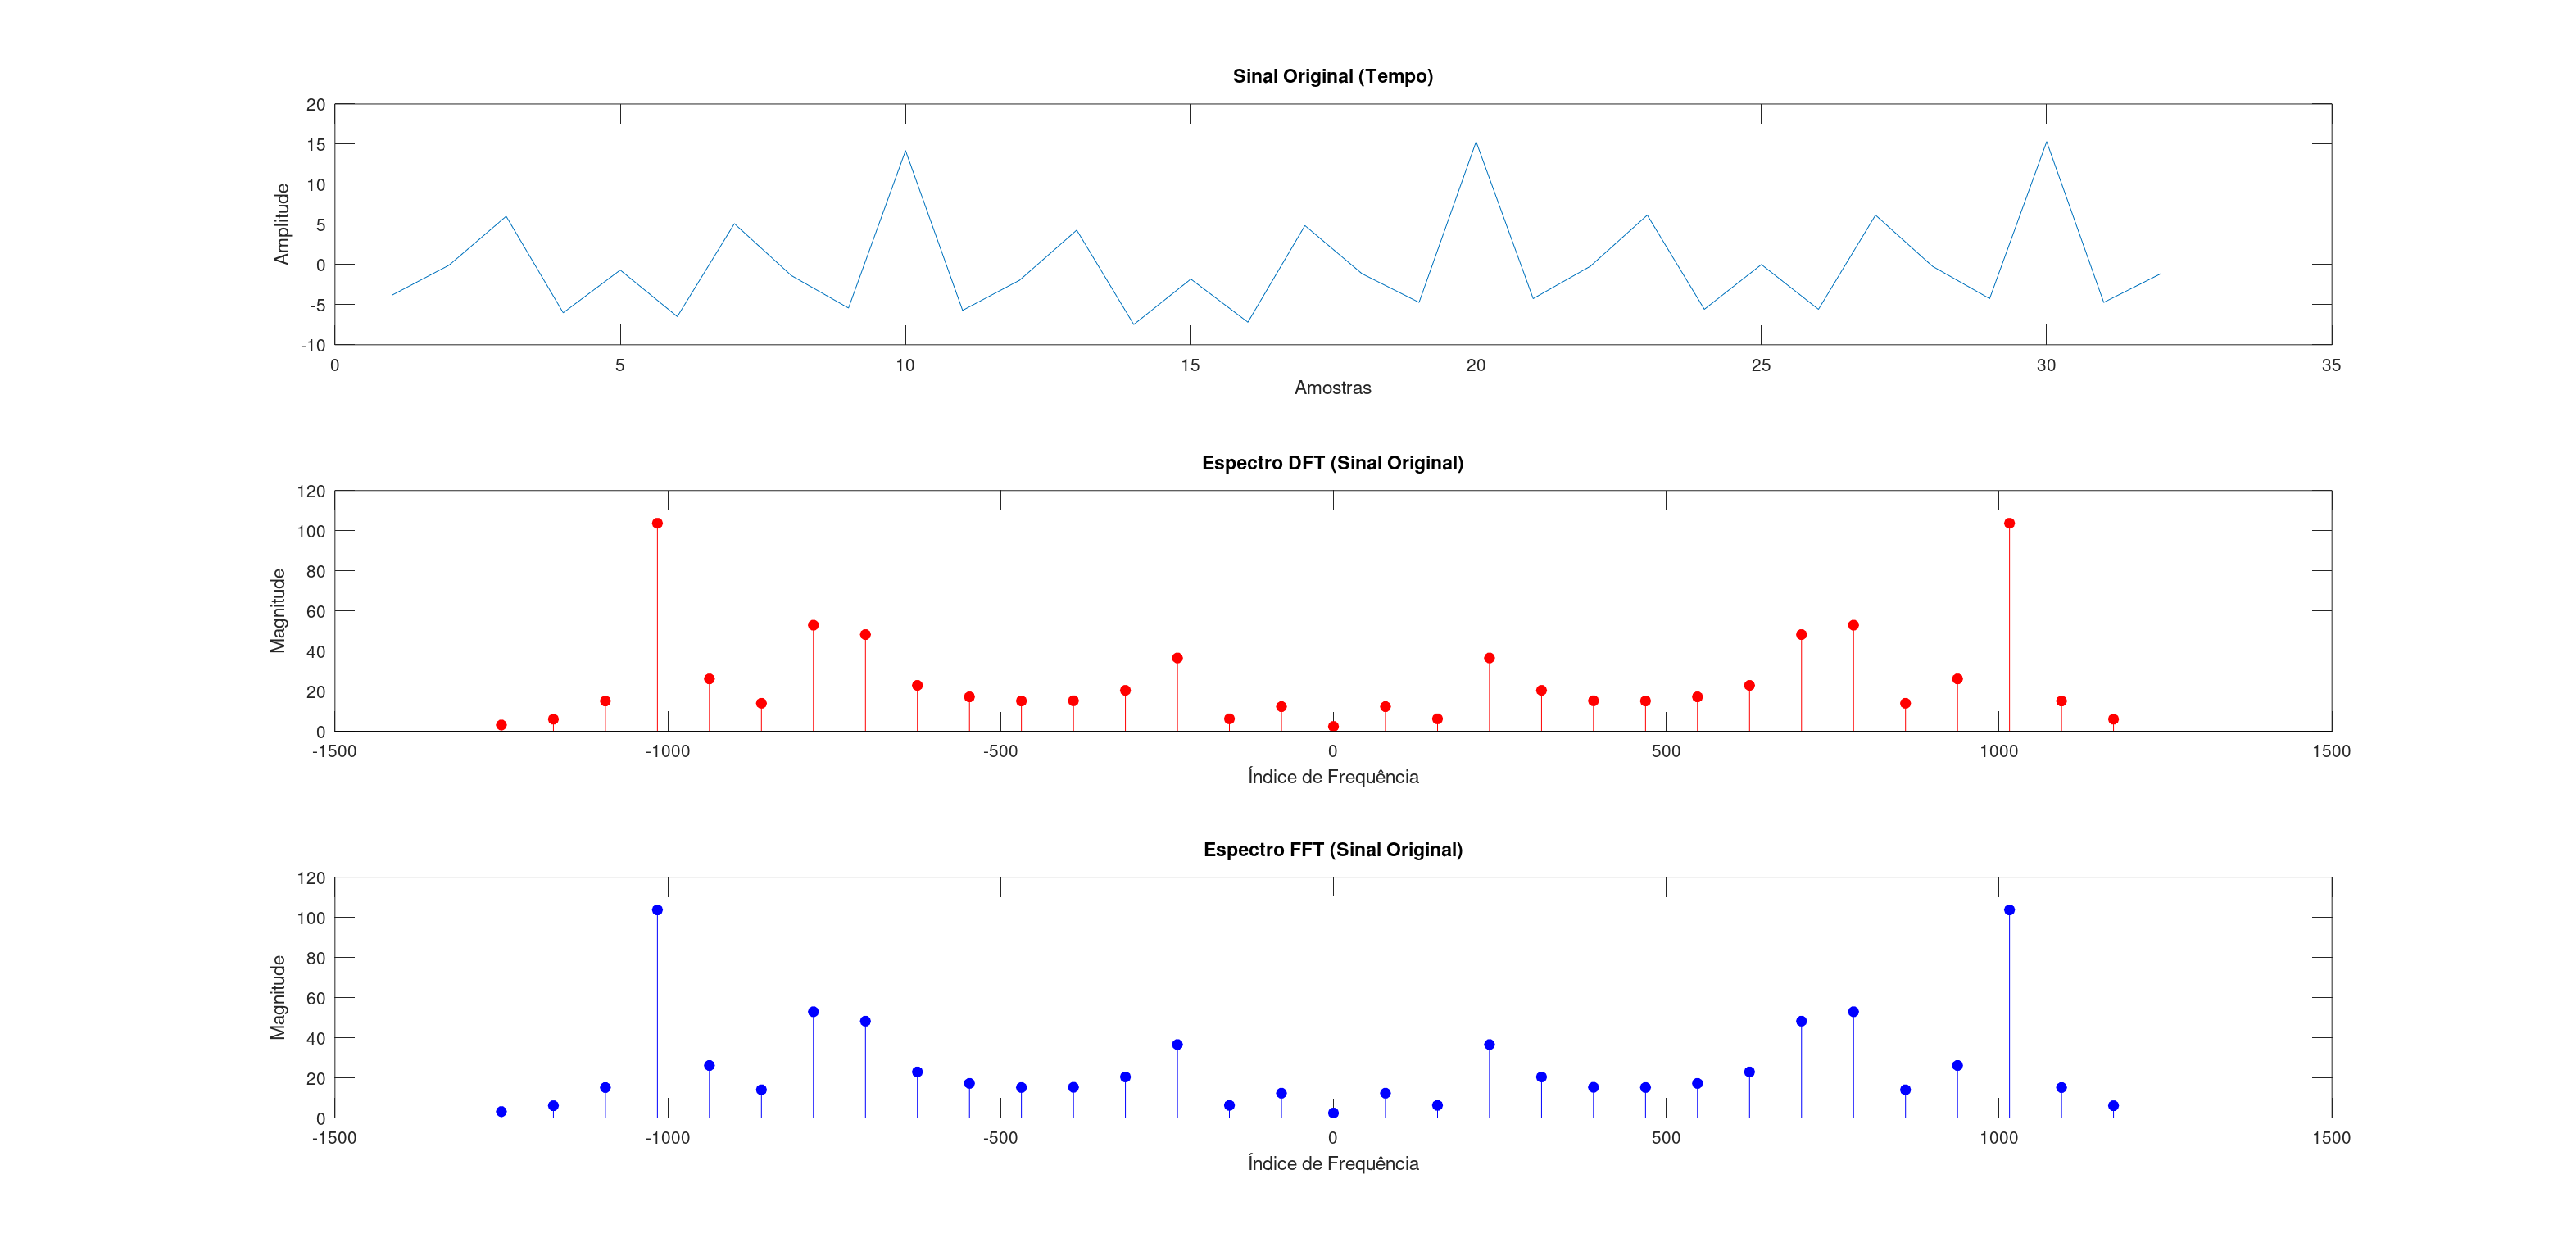
\includegraphics[width=1\linewidth]{03_experimental_analysis/plot_results/32_samples_dft_fft.png}
    \caption{DFT+FFT Aplicada a 32 amostras}
    \label{fig:signal_32samples_fft-dft}
\end{figure}

%%%%%%%%%%%%%%%%%%%%%%%%%%%%%%%%%%%%%%%%%%%%%%%%%%%%%%%%%%%%%%%%%%%%%%
\subsubsection*{(b) \textbf{(1,0 pontos)}}
Aumente o comprimento do item anterior para 64 amostras, aumentando 32 zeros à direita das amostras originais. Calcule a DFT e FFT. Compare com o item anterior e comente seus resultados.

\begin{figure}[H]
    \centering
    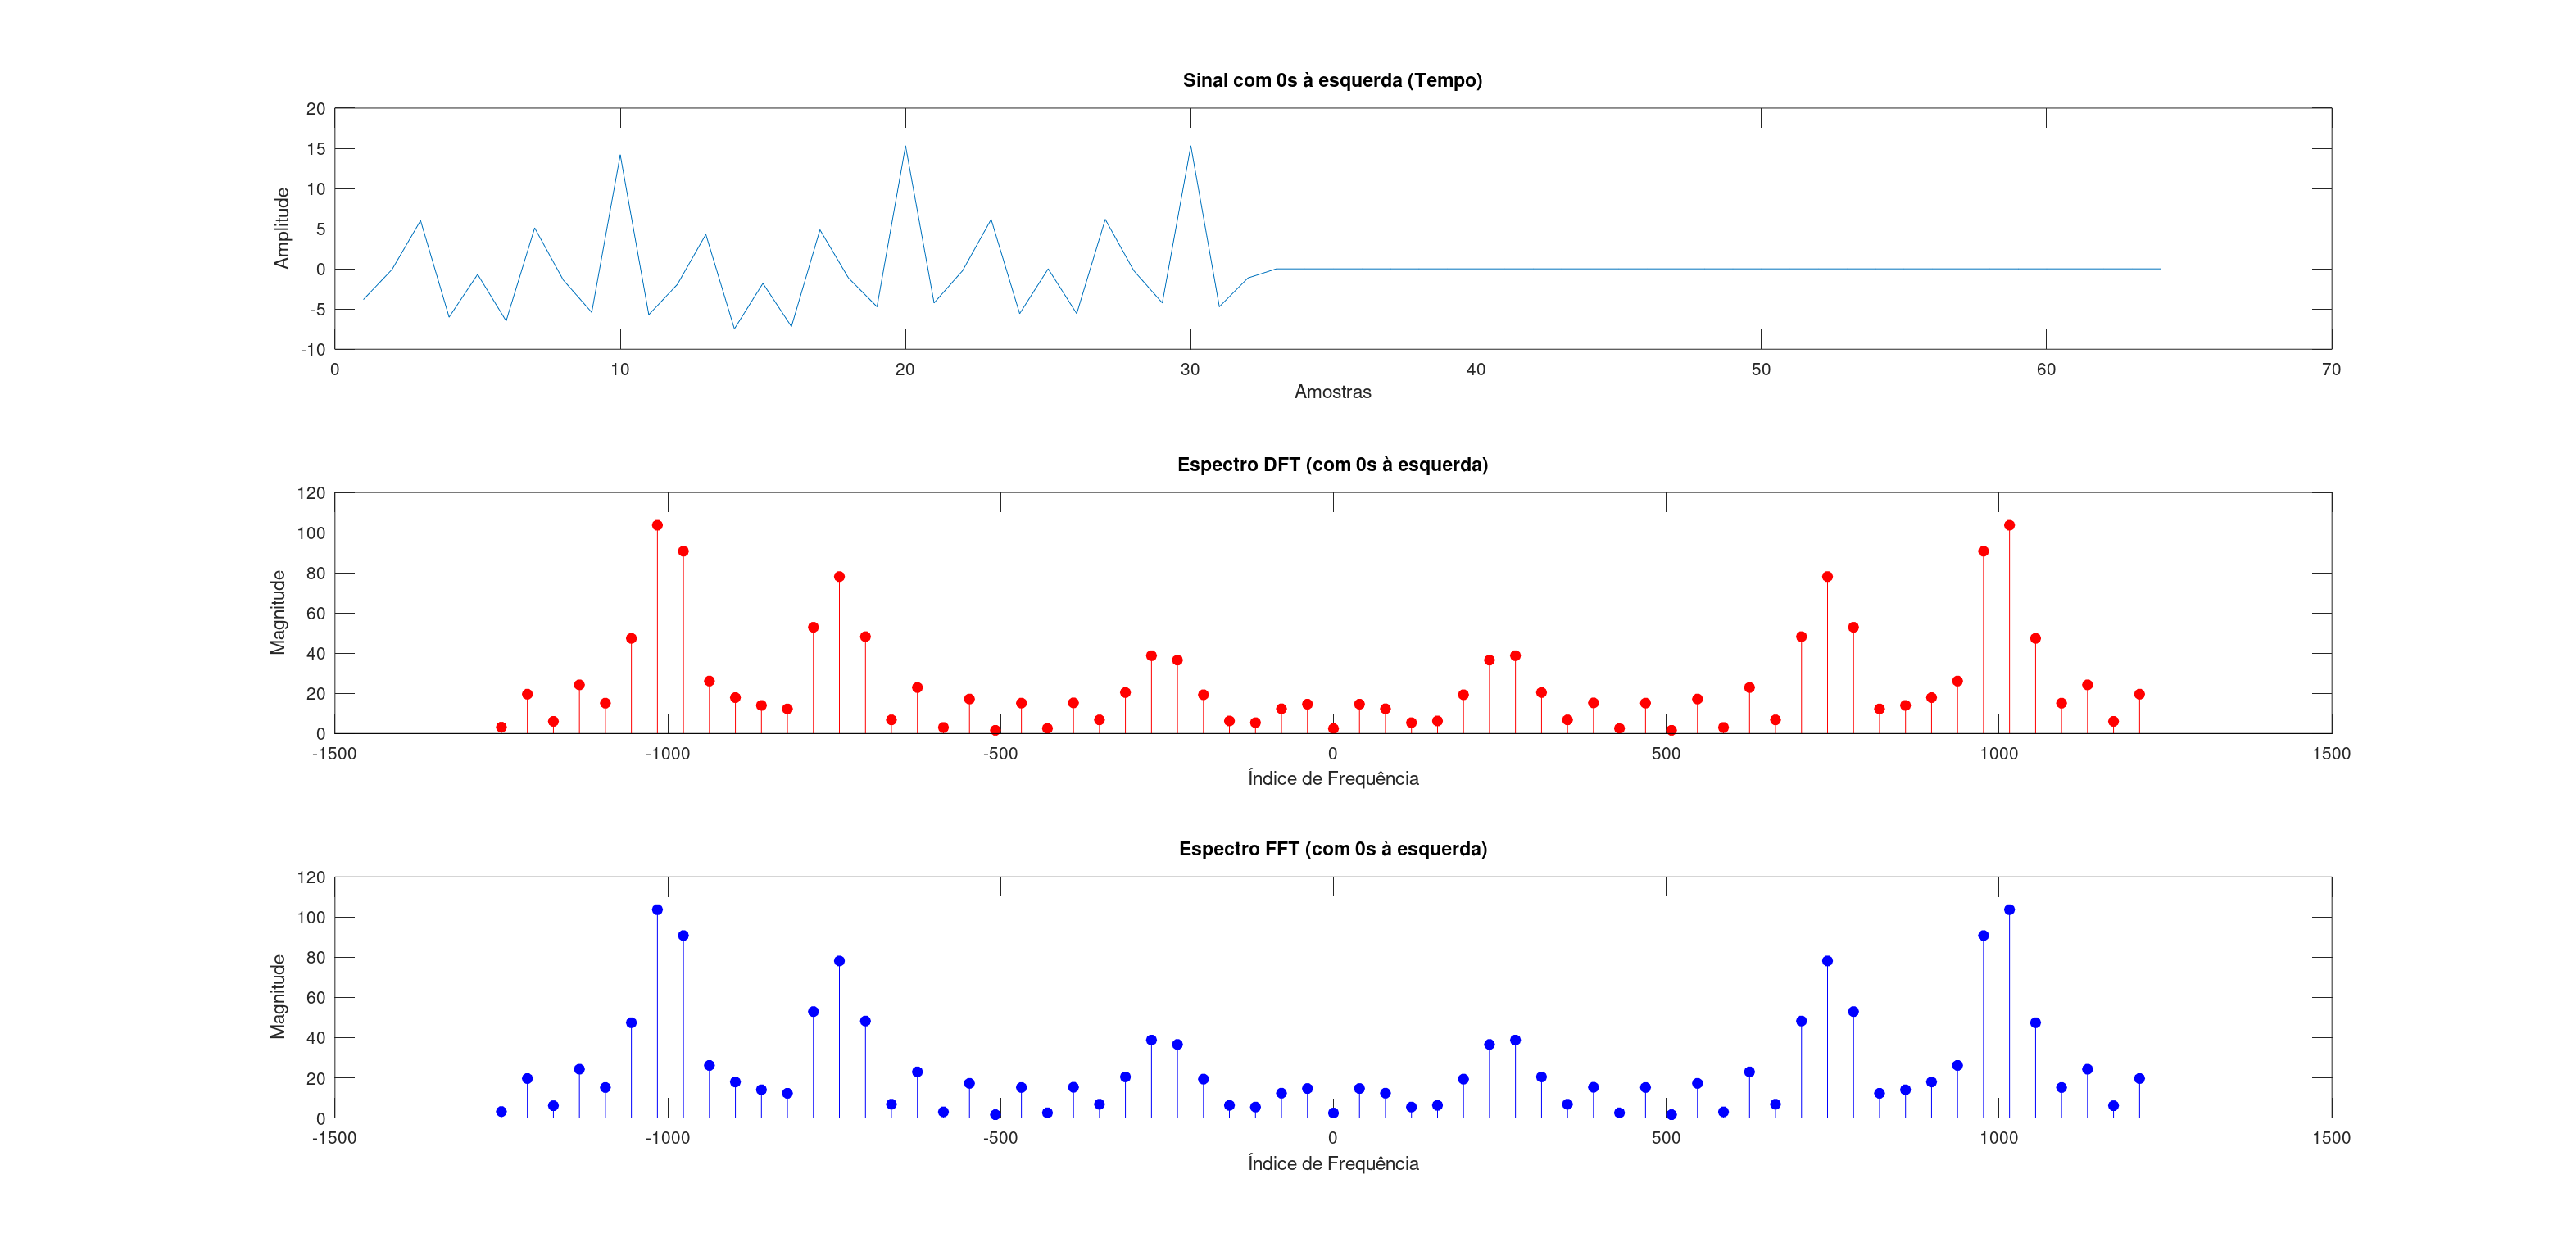
\includegraphics[width=1\linewidth]{03_experimental_analysis/plot_results/32_samples_dft_fft_padded.png}
    \caption{DFT+FFT Aplicada a 32 amostras com 32 zeros à direita}
    \label{fig:signal_32samples_fft-dft_padded}
\end{figure}

%%%%%%%%%%%%%%%%%%%%%%%%%%%%%%%%%%%%%%%%%%%%%%%%%%%%%%%%%%%%%%%%%%%%%%
\subsubsection*{(c) \textbf{(1,0 pontos)}}
Calcule a DFT e FFT usando uma janela de 64 amostras. É possivel observar no espectro as senóides?

%%%%%%%%%%%%%%%%%%%%%%%%%%%%%%%%%%%%%%%%%%%%%%%%%%%%%%%%%%%%%%%%%%%%%%
\subsubsection*{(d) \textbf{(1,0 pontos)}}
Aumente o comprimento do item anterior para 128 amostras, aumentando 64 zeros à direita das amostras originais. Calcule a DFT e FFT. Compare com o item anterior e comente seus resultados.

%%%%%%%%%%%%%%%%%%%%%%%%%%%%%%%%%%%%%%%%%%%%%%%%%%%%%%%%%%%%%%%%%%%%%%
\subsubsection*{(e) \textbf{(1,0 pontos)}}
E assim por diante, repita os ítens (a) e (b) para 256, 512 e 1024 amostras do sinal.

%%%%%%%%%%%%%%%%%%%%%%%%%%%%%%%%%%%%%%%%%%%%%%%%%%%%%%%%%%%%%%%%%%%%%%
\subsubsection*{(f) \textbf{(1,0 pontos)}}
Monte numa tabela comparativa a quantidade de operações (produtos e somas) realizadas.

